\documentclass[11pt]{article}

\newcommand{\yourname}{Kevin Zhang}

\def\comments{0}

%format and packages

%\usepackage{algorithm, algorithmic}
\usepackage{forest}
\usepackage{tikz}
\usepackage{algpseudocode}
\usepackage{amsmath, amssymb, amsthm}
\usepackage{tcolorbox}
\usepackage{enumerate}
\usepackage{enumitem}
\usepackage{framed}
\usepackage{verbatim}
\usepackage[margin=1.0in]{geometry}
\usepackage{microtype}
\usepackage{kpfonts}
\usepackage{palatino}
	\DeclareMathAlphabet{\mathtt}{OT1}{cmtt}{m}{n}
	\SetMathAlphabet{\mathtt}{bold}{OT1}{cmtt}{bx}{n}
	\DeclareMathAlphabet{\mathsf}{OT1}{cmss}{m}{n}
	\SetMathAlphabet{\mathsf}{bold}{OT1}{cmss}{bx}{n}
	\renewcommand*\ttdefault{cmtt}
	\renewcommand*\sfdefault{cmss}
	\renewcommand{\baselinestretch}{1.06}

\usepackage[boxruled,vlined,nofillcomment]{algorithm2e}
	\SetKwProg{Fn}{Function}{\string:}{}
	\SetKwFor{While}{While}{}{}
	\SetKwFor{For}{For}{}{}
	\SetKwIF{If}{ElseIf}{Else}{If}{:}{ElseIf}{Else}{:}
	\SetKw{Return}{Return}
	

%enclosure macros
\newcommand{\paren}[1]{\ensuremath{\left( {#1} \right)}}
\newcommand{\bracket}[1]{\ensuremath{\left\{ {#1} \right\}}}
\renewcommand{\sb}[1]{\ensuremath{\left[ {#1} \right\]}}
\newcommand{\ab}[1]{\ensuremath{\left\langle {#1} \right\rangle}}

%probability macros
\newcommand{\ex}[2]{{\ifx&#1& \mathbb{E} \else \underset{#1}{\mathbb{E}} \fi \left[#2\right]}}
\newcommand{\pr}[2]{{\ifx&#1& \mathbb{P} \else \underset{#1}{\mathbb{P}} \fi \left[#2\right]}}
\newcommand{\var}[2]{{\ifx&#1& \mathrm{Var} \else \underset{#1}{\mathrm{Var}} \fi \left[#2\right]}}

%useful CS macros
\newcommand{\poly}{\mathrm{poly}}
\newcommand{\polylog}{\mathrm{polylog}}
\newcommand{\zo}{\{0,1\}}
\newcommand{\pmo}{\{\pm1\}}
\newcommand{\getsr}{\gets_{\mbox{\tiny R}}}
\newcommand{\card}[1]{\left| #1 \right|}
\newcommand{\set}[1]{\left\{#1\right\}}
\newcommand{\negl}{\mathrm{negl}}
\newcommand{\eps}{\varepsilon}
\DeclareMathOperator*{\argmin}{arg\,min}
\DeclareMathOperator*{\argmax}{arg\,max}
\newcommand{\eqand}{\qquad \textrm{and} \qquad}
\newcommand{\ind}[1]{\mathbb{I}\{#1\}}
\newcommand{\sslash}{\ensuremath{\mathbin{/\mkern-3mu/}}}
\newcommand{\pipe}{\hspace{3pt}|\hspace{3pt}}

%mathbb
\newcommand{\N}{\mathbb{N}}
\newcommand{\R}{\mathbb{R}}
\newcommand{\Z}{\mathbb{Z}}
%mathcal
\newcommand{\cA}{\mathcal{A}}
\newcommand{\cB}{\mathcal{B}}
\newcommand{\cC}{\mathcal{C}}
\newcommand{\cD}{\mathcal{D}}
\newcommand{\cE}{\mathcal{E}}
\newcommand{\cF}{\mathcal{F}}
\newcommand{\cL}{\mathcal{L}}
\newcommand{\cM}{\mathcal{M}}
\newcommand{\cO}{\mathcal{O}}
\newcommand{\cP}{\mathcal{P}}
\newcommand{\cQ}{\mathcal{Q}}
\newcommand{\cR}{\mathcal{R}}
\newcommand{\cS}{\mathcal{S}}
\newcommand{\cU}{\mathcal{U}}
\newcommand{\cV}{\mathcal{V}}
\newcommand{\cW}{\mathcal{W}}
\newcommand{\cX}{\mathcal{X}}
\newcommand{\cY}{\mathcal{Y}}
\newcommand{\cZ}{\mathcal{Z}}

%theorem macros
\newtheorem{thm}{Theorem}
\newtheorem{lem}[thm]{Lemma}
\newtheorem{fact}[thm]{Fact}
\newtheorem{clm}[thm]{Claim}
\newtheorem{rem}[thm]{Remark}
\newtheorem{coro}[thm]{Corollary}
\newtheorem{prop}[thm]{Proposition}
\newtheorem{conj}[thm]{Conjecture}

\theoremstyle{definition}
\newtheorem{defn}[thm]{Definition}
\newtheoremstyle{case}{}{}{}{}{}{:}{ }{}
\theoremstyle{case}
\newtheorem{case}{Case}

\theoremstyle{theorem}
\newtheorem{prob}{Problem}
\newtheorem{sol}{Solution}

\tikzset{every picture/.style={line width=0.75pt}} %set default line width to 0.75pt        

\begin{document}
{\large
\noindent Name: \yourname}

\vspace{15pt}

% Problem 1
\begin{prob}
\end{prob}

Consider convex function $f : \R^n \longrightarrow \R$ and a convex set $S$.

\begin{enumerate}[label=(\alph*)]

% Part A
\item Show that the set of minimizers of $f$ over $S$ is convex. 

Assume for the sake of contradiction that the set of minimizers $M$ is not convex. 
What this means is there is a least one point $x_c \notin M$ and two points $x_1, x_2 \in M$ 
such that $x_c$ is between $x_1$ and $x_2$. 

From convexity of $f$, we have that $f(\theta x_1 + (1 - \theta) x_2) \leq \theta f(x_1) + (1 - \theta) f(x_2)$. 
From lecture, we know that for convex $f$ and convex $S$, any local minimum is also a global minimum. Thus $f(x_1) = f(x_2)$.
Combining all of these together (and that $x_c$ is between $x_1$ and $x_2$):

\begin{align*}
f(\theta x_1 + (1 - \theta) x_2) &\leq \theta f(x_1) + (1 - \theta) f(x_2) \\
f(\theta x_1 + (1 - \theta) x_2) &\leq \theta f(x_1) + (1 - \theta) f(x_1) \\
f(x_c) &\leq f(x_1) \\
\end{align*}

So $x_c$ is a minimizer. But $x_c \notin M$, and $M$ is the set of minimizers. So by contradiction, $M$ must be convex.

% Part B
\item Give counterexample if $f$ is not convex.

\begin{figure}[h!]
  \centering
  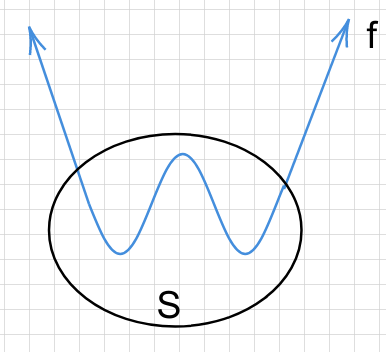
\includegraphics[totalheight=3cm]{images/f-not-convex.png}
\end{figure}

It's easy to see from the figure that even if two points $x_1, x_2$ are minimizers, not
all points between the points would be minimizers. Thus, $M$ cannot be convex.

% Part C
\item Give counterexample if $S$ is not convex.

\begin{figure}[h!]
  \centering
  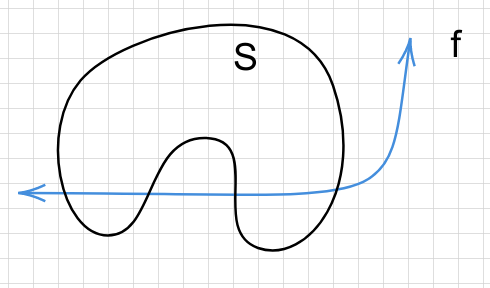
\includegraphics[totalheight=3cm]{images/s-not-convex.png}
\end{figure}

From the figure, the set of minimizers has been split because $S$ is not convex. It is easy 
to see that there would be some minimizers for $f$ that don't end up in $S$. Thus, $M$ cannot
be convex.

\end{enumerate}

\newpage

% Problem 2
\begin{prob}
\end{prob}

Goal is to find $x$ that minimizes $f(x) = \frac{1}{2} ||Ax - b||^2$.

\begin{enumerate}[label=(\alph*)]

% Part A
\item We want to prove $f$ is convex. 

This can be done by showing $f(y) - f(x) \geq \langle \nabla f(x), y - x \rangle$. 
With $\nabla f(x) = A^T ||Ax - b||$, we can expand the expression:

\begin{align*}
f(y) - f(x) &\underset{\geq}{?} \langle \nabla f(x), y - x \rangle \\
\frac{1}{2} ||Ay - b||^2 - \frac{1}{2} ||Ax - b||^2 &\underset{\geq}{?} \langle A^T ||Ax - b||, y - x \rangle \\
\frac{1}{2} \left( ||Ay - b||^2 - ||Ax - b||^2 \right) &\underset{\geq}{?} \langle A^T ||Ax - b||, y - x \rangle \\
\frac{1}{2} \langle Ay - Ax, (Ay - b) + (Ax - b) \rangle &\underset{\geq}{?} \langle A^T ||Ax - b||, y - x \rangle \\
\frac{1}{2} A^T \langle y - x, (Ay - b) + (Ax - b) \rangle &\underset{\geq}{?} A^T \langle ||Ax - b||, y - x \rangle \\
\langle y - x, (Ay - b) + (Ax - b) \rangle &\underset{\geq}{?} 2 \langle Ax - b, y - x \rangle \\
\end{align*}

At this point, we need to do a bit of case analysis to divide by $y - x$. If $y - x < 0$, we need to flip the sign. So,
for Case 1 ($y - x > 0$), we have:

\begin{align*}
(Ay - b) + (Ax - b) \rangle &\underset{\geq}{?} 2(Ax - b) \\
(Ay - b) \rangle &\geq (Ax - b) \\
\end{align*}

And for Case 2($y - x < 0$), we have:

\begin{align*}
(Ay - b) + (Ax - b) \rangle &\underset{\leq}{?} 2(Ax - b) \\
(Ay - b) \rangle &\leq (Ax - b) \\
\end{align*}

Thus, $f$ is convex.

% Part B
\item Prove that $f$ is $\beta$-smooth for as small $\beta$ as you can. We can do this by examining the 
definition for $\beta$-smoothness:

\begin{align*}
|| \nabla f(x) - \nabla f(y) || &\leq \beta ||x - y|| \\
\left|\left| A^T || Ax - b ||  - A^T || Ay - b || \right|\right| &\leq \beta ||x - y|| \\
|| A^T || || Ax -b - (Ay - b) || &\leq \beta ||x - y|| \\
|| A^T || || Ax - Ay || &\leq \beta ||x - y|| \\
|| A^T A || || x - y || &\leq \beta ||x - y|| \\
|| A^T A || &\leq \beta \\
\end{align*}

We have that $\beta \geq ||A^T A||_2$, which is the equivalent of $\beta \geq ||A||_2^2$.

% Part C
\item Consider matrix $M = I - \gamma A^T A$ for some constant $\gamma$. We want to use gradient descent
algorithm with $x^{(t)} \longleftarrow M(x^{(t-1)} - x^*) + x^*$. We want to pick $\gamma$ such that $x^{(t)}$ 
converges to $x^*$.

We can expand out $x^{(t)}$, since we know it should converge to $x^*$.

\begin{align*}
x^{(t)} &\longleftarrow M(x^{(t-1)} - x^*) + x^* \\
x^{(t)} &\longleftarrow (I - \gamma(A^T A))(x^{(t-1)} - x^*) + x^* \\
x^{(t)} &\longleftarrow (I - \gamma(A^T A))(x^{(t-1)}) - (I - \gamma(A^T A))(x^*) + x^* \\
x^{(t)} &\longleftarrow x^{(t-1)} - (\gamma(A^T A))(x^{(t-1)}) - x^* + (\gamma(A^T A))(x^*) + x^* \\
x^{(t)} &\longleftarrow x^{(t-1)} - (\gamma(A^T A))(x^{(t-1)}) + (\gamma(A^T A))(x^*)\\
\end{align*}

Since we want to convege to $x^*$, $x^{(t-1)} - (\gamma(A^T A))(x^{(t-1)})$ should zero out, and
the rest of the term should equal $x^*$. Conveniently, the rest of the term is $(\gamma(A^T A))(x^*)$, so
if we let $\gamma = \frac{1}{||A^T A||_2} = \frac{1}{||A||_2^2}$, we can accomplish both.

TODO: Find the bound

\end{enumerate}

\newpage

% Problem 3 
\begin{prob}
\end{prob}

Our goal is to find the first singular vector $v_1$ of a given matrix $A$. This is done by finding a vector $x$
that minimizes $f(x) = - \frac{1}{2} ||Ax||^2$. We can assume a starting point $x^{(0)}$ such that 
$\langle x^{(0)}, v_1 \rangle \geq \alpha$. 

\begin{enumerate}[label=(\alph*)]

% Part A
\item State a projected gradient descent algorithm with fixed size $\eta$.

The key idea here is to move along with the gradient, and then project back onto $f(x)$. The projection in this
case is to normalize the vector, because we're looking for a vector of length 1. The algorithm is
the gradient descent algorithm as follows ($\nabla f(x) = - A^T A$): 

$y^{(t)} \longleftarrow x^{(t-1)} - \eta \nabla f(x^{(t-1)})$

$x^{(t)} \longleftarrow y^{(t)} / || y^{(t)} ||$

% Part B
\item Let $\eta \geq 1/\sigma_1^2$ and $z^{(t)}$ be the projection of $x^{(t)}$ onto the span of singular vectors with
singular values less than $(1 - \varepsilon)\sigma_1$. Show that after $t = O(\frac{ln(1 / \varepsilon \alpha)}{\varepsilon})$ steps, 
we have $||z^{(t)}|| \leq \varepsilon$.

We can express $y^{(t)}$ as $(1 + \eta A^T A) x ^{(t-1)}$. If we let $M = (1 + \eta A^T A)$, then
after $t$ time steps, $||z^{(t)}|| = (M^t x^{(0)}) / || M^t x^{(0)} ||$. If we plug in the span of singular vectors 
for $A$, we get the following (NOTE: I worked with Michael to arrive on this):

\begin{align*}
\left( (M^t x^{(0)}) / || M^t x^{(0)} || \right)^2 &= \frac{(1 + \eta (1 - \varepsilon) \sigma_1^2)^{2t}}{(1 + \eta \sigma_1^2)^{2t} \alpha} \\  
|| z^{(t)} || &= \frac{(1 + (1 - \varepsilon))^{t}}{(2)^{t} \alpha} \\  
\end{align*}

We can then solve for $t$:

\begin{align*}
|| z^{(t)} || &\leq \varepsilon \\
\frac{(1 + (1 - \varepsilon))^{t}}{(2)^{t} \alpha} \leq \varepsilon \\
(2 - \varepsilon)^t \leq \varepsilon \alpha \\
e^{t \varepsilon/2} \geq (1 / \varepsilon \alpha) \\
t \geq \frac{\ln{ 2 / \varepsilon \alpha}}{\varepsilon} \\
\end{align*}

Thus, $t$ is $O(\frac{ln(1 / \varepsilon \alpha)}{\varepsilon})$.

\end{enumerate}

\newpage

% Problem 4
\begin{prob}
\end{prob}

We have an $\alpha$-strongly convex $f(x)$, over bounded domain $S$. Assume that $||\nabla f(x)|| \leq G \forall x \in S$. 
We'll use the projected gradient descent algorithm:

$y^{(t)} \longleftarrow x^{(t-1)} - \eta_t \nabla f(x^{(t-1)})$ 

$x^{(t)} \longleftarrow \argmin{x \in S} ||x - y^{(t)}||^2 / 2$

\begin{enumerate}[label=(\alph*)]

\item Prove the following:

$\Delta_t = \left(f(x^{(t-1)} - f(x^*)) + \frac{\alpha}{2} ||x^{(t-1)} - x^*||^2 \right) + \frac{1}{2 \eta_t} \left( ||x^{(t)} - x^* || - ||x^{(t-1)} - x^*||^2 \right) \leq \frac{\eta_t G^2}{2}$.

We can do so by examining the two summands separately, and then combining the results. 

First, the left summand. We can use the $\alpha$-convexity to bound this term. From the definition of 
$\alpha$-convexity, and if we let $y = x^*$ and $x = x^{(t-1)}$, we get the following:

\begin{align*}
f(y) - f(x) &\geq \langle \nabla f(x), y -x \rangle + \frac{\alpha}{2} ||y - x||^2 \\
f(x^*) - f(x^{(t-1)}) &\geq \langle \nabla f(x^{(t-1)}), x^* -x^{(t-1)} \rangle + \frac{\alpha}{2} ||x^* - x^{(t-1)}||^2 \\
f(x^*) - f(x^{(t-1)}) - \frac{\alpha}{2} ||x^* - x^{(t-1)}||^2 &\geq \langle \nabla f(x^{(t-1)}), x^* -x^{(t-1)} \rangle \\
f(x^{(t-1)}) - f(x^*) + \frac{\alpha}{2} ||x^* - x^{(t-1)}||^2 &\leq - \langle \nabla f(x^{(t-1)}), x^* -x^{(t-1)} \rangle \\
\end{align*}

Next, we can break down the right summand.

\begin{align*}
RS &= \frac{1}{2 \eta_t} \left( ||x^{(t)} - x^* || - ||x^{(t-1)} - x^*||^2 \right) \\ 
   &= \frac{1}{2 \eta_t} \langle x^{(t)} - x^{(t-1)},  x^{(t)} + x^{(t-1)} - 2 x^* \rangle \\ 
   &\leq \frac{1}{2 \eta_t} \langle y^{(t)} - x^{(t-1)},  y^{(t)} + x^{(t-1)} - 2 x^* \rangle \\ 
   &= \frac{1}{2 \eta_t} \langle - \eta_t \nabla f(x^{(t-1)}), - \eta_t \nabla f(x^{(t-1)}) + 2 x^{(t-1)} - 2 x^* \rangle \\ 
   &= \frac{1}{2 \eta_t} \left( \eta_t^2 (\nabla f(x^{(t-1)}))^2 + 2\eta_t \langle \nabla f(x^{(t-1)}), x^* - x^{(t-1)} \rangle \right)\\ 
   &= \frac{\eta_t}{2} (\nabla f(x^{(t-1)}))^2 + \langle \nabla f(x^{(t-1)}), x^* - x^{(t-1)} \rangle\\ 
\end{align*}

Combining the two terms, and subsituting $(\nabla f(x^{(t-1)}))^2 \leq G$, we get the following:

\begin{align*}
\left(- \langle \nabla f(x^{(t-1)}), x^* -x^{(t-1)} \rangle \right) &+ \left( \frac{\eta_t}{2} (\nabla f(x^{(t-1)}))^2 + \langle \nabla f(x^{(t-1)}), x^* - x^{(t-1)} \rangle \right) \\
\frac{\eta_t}{2} &(\nabla f(x^{(t-1)}))^2 \\
&\frac{\eta_t G^2}{2}
\end{align*}

\item We want to design the coefficients of $a_t$ and $\eta_t$ such that for $\sum_{t=1}^{T} a_t \Delta_t$, the coefficents of $||x^{(t)} - x^*||^2$ cancel out. 
We also want to find the bound of the resulting gradient descent algorithm. 

If we examine $\Delta_t$ closely over the sum of $a_t$, and attempt to express $a_t$ in terms of $a_{t-1}$, we get following:

$\sum_{t=1}^{T} a_t \Delta_t = ... + a_{t-1} \left( \frac{1}{2 \eta_t} || x^{t-1} - x^* ||^2 \right) + ... + a_t \left( \frac{\alpha}{2} || x^{t-1} - x^* ||^2 \right) - a_t \left( \frac{1}{2 \eta_t} || x^{t-1} - x^* ||^2 \right) + ... $

\begin{align*}
a_{t-1} (\frac{1}{2 \eta_t}) &= a_{t} (\frac{\alpha}{2} - \frac{1}{2 \eta_t}) \\
a_{t} &= a_{t-1} \left( \frac{(\frac{1}{2 \eta_t})}{\frac{\alpha}{2} - \frac{1}{2 \eta_t}} \right) \\
a_{t} &= a_{t-1} \left( \frac{1}{\eta_t \alpha - 1}\right) \\
\end{align*}

Next, we can examine the sum to determine $a_0$ and $\eta_t$:

\begin{align*}
\sum_{t=1}^{T} a_t \Delta_t &\leq \sum_{t=1}^{T} a_t \frac{\eta_t G^2}{2} \\
T(f(\bar{x}) - f(x^*)) - \frac{a_T}{2 \eta_t} || x^{T} - x^* ||^2 + \frac{a_0 \alpha}{2} || x^{0} - x^* ||^2 &\leq (\frac{1}{\eta_t \alpha - 1})^{(T)(T+1)/2} \frac{T a_0 \eta_t G^2}{2} \\
\end{align*}

Note: Not exactly sure how to proceed from here.

\end{enumerate}

\end{document}
